\chapter{System Analysis \& Design}

\section{Introduction}
This chapter delineates the formal requirements engineering and architectural design of the Kemora platform. A robust system design is the foundation of any scalable application, ensuring that the software not only meets its current functional objectives but is also resilient to future expansion and varying loads. The architecture utilizes ASP.NET Core for the backend API and Flutter for the cross-platform mobile frontend.

\section{Requirements Specification}

\subsection{Functional Requirements}
Functional requirements define the specific behaviors and functions the system must perform. The core functional requirements for Kemora are:
\begin{itemize}
    \item \textbf{FR1 - User Authentication \& Authorization:} The system must allow users to register, log in (via email/password or Google OAuth), and securely manage their sessions. Authentication is handled via JWT tokens, with support for token refresh, email confirmation, and password reset functionalities.
    \item \textbf{FR2 - Destination Discovery:} The system must display a categorized directory of Egyptian governorates and specific tourist attractions, augmented with images (via Cloudinary) and metadata (via Google Places).
    \item \textbf{FR3 - AI Trip Generation:} The system must accept user parameters (duration, budget, preferences) and generate a logically ordered, day-by-day itinerary using an external LLM (via OpenRouter).
    \item \textbf{FR4 - Trip Modification (Custom Roadmap):} Users must be able to view their generated trips on an interactive map, manually add places, remove places, and reorder itinerary items dynamically.
    \item \textbf{FR5 - Social Networking \& Community:} The system must provide a community feed where users can publish posts, attach media, leave comments, and react to content. Posts can be directly linked to user-generated AI trips.
    \item \textbf{FR6 - Gamification Engine:} The system must track user actions and automatically award points and badges (e.g., "AiPioneer", "CityHopper") upon crossing specific thresholds.
\end{itemize}

\subsection{Non-Functional Requirements}
Non-functional requirements specify criteria that judge the operation of the system, guaranteeing stability, security, and high performance.
\begin{itemize}
    \item \textbf{NFR1 - Performance \& Caching:} The backend API must respond to standard data retrieval requests in under 100ms under normal load. AI generation requests should resolve within 15 seconds. To achieve this, the system uses in-memory caching (\texttt{MemoryCacheService}) for frequent queries and caches available LLM models concurrently.
    \item \textbf{NFR2 - Scalability:} The architecture must support stateless scaling. Session state must not be stored in server memory. JWTs ensure that requests can be routed to any backend node behind a load balancer. Thread-safe operations (using \texttt{SemaphoreSlim}) ensure safe initialization of singletons like the OpenRouter model cache under high load.
    \item \textbf{NFR3 - Security Protocols:}
    \begin{itemize}
        \item \textbf{Data Encryption:} All communication is encrypted via TLS 1.2/1.3.
        \item \textbf{Password Hashing:} Passwords are cryptographically hashed using PBKDF2 (the ASP.NET Core Identity default) with a high iteration count.
        \item \textbf{JWT Structure:} JSON Web Tokens are signed using the HMAC-SHA512 algorithm (\texttt{SecurityAlgorithms.HmacSha512Signature}). Tokens contain specific claims (\texttt{NameId}, \texttt{Email}, \texttt{GivenName}, \texttt{Role}) and possess a 7-day expiration time to balance user convenience with security. Refresh tokens are generated as 32-byte cryptographically secure random numbers encoded in Base64.
        \item \textbf{Rate Limiting:} Critical endpoints (e.g., \texttt{AuthController}) are protected against brute-force and DDoS attacks via ASP.NET Core Rate Limiting (\texttt{[EnableRateLimiting("auth")]}).
    \end{itemize}
    \item \textbf{NFR4 - Maintainability:} The backend strictly adheres to Clean Architecture. The Domain layer is completely independent of external frameworks. Application logic is separated into Services (\texttt{TripService}, \texttt{TripPlannerService}), while external integrations reside in the Infrastructure layer (\texttt{AuthService}, \texttt{OpenRouterAiService}). HTTP routing is confined to the API tier (\texttt{TripsController}, \texttt{AuthController}, \texttt{PlacesController}).
\end{itemize}

\section{System Architecture}
Kemora utilizes a multi-tier, decoupled architecture designed for high cohesion and loose coupling. The backend is structured into four main layers: API, Application, Domain, and Infrastructure.

\subsection{Architectural Layers}
\begin{enumerate}
    \item \textbf{Domain Layer:} Contains core business entities (\texttt{ApplicationUser}, \texttt{Trip}, \texttt{Place}) and repository interfaces.
    \item \textbf{Application Layer:} Houses Data Transfer Objects (DTOs), business service interfaces (\texttt{ITripService}, \texttt{IAiService}), and core business logic (\texttt{TripService}, \texttt{TripPlannerService}).
    \item \textbf{Infrastructure Layer:} Implements the interfaces. Key implementations include \texttt{TokenService} for JWT handling, \texttt{OpenRouterAiService} for communicating with LLMs, and \texttt{CloudinaryImageService} for media storage.
    \item \textbf{API Layer:} Exposes RESTful endpoints (e.g., \texttt{AuthController}, \texttt{TripsController}) secured via Bearer authentication.
\end{enumerate}

\begin{figure}[H]
    \centering
    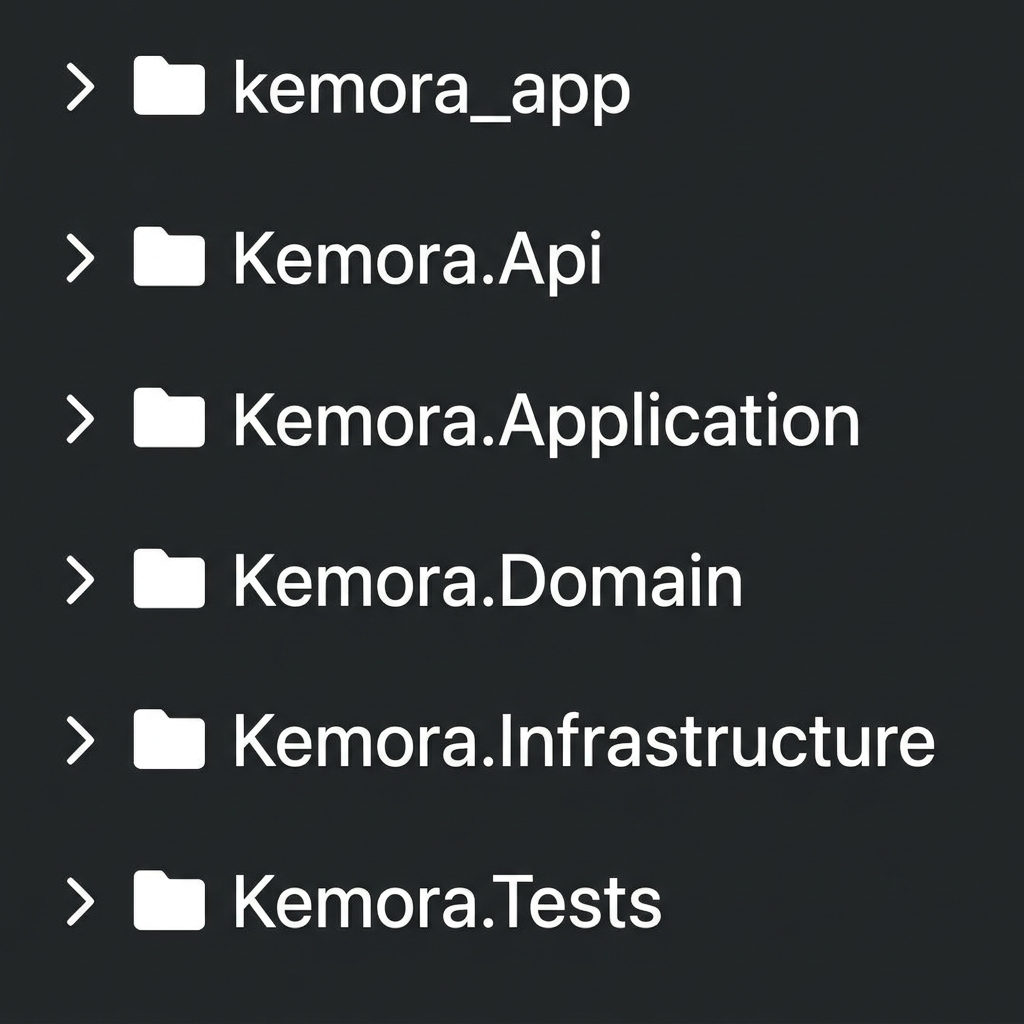
\includegraphics[width=0.9\textwidth]{figures/architecture.png}
    \caption{Kemora's Overall Architecture}
    \label{fig:architecture}
\end{figure}

\subsection{Sequence Diagrams}

\subsubsection{Authentication Flow (JWT Generation)}
The following Mermaid sequence diagram illustrates the login and token generation process when a user authenticates via the \texttt{AuthController}.

\begin{verbatim}
sequenceDiagram
    participant Client as Flutter App
    participant API as AuthController
    participant AuthSvc as AuthService
    participant SignIn as SignInManager
    participant Identity as UserManager
    participant TokenSvc as TokenService
    participant DB as SQL Server

    Client->>API: POST /api/v1/auth/login (email, password)
    API->>AuthSvc: LoginAsync(model)
    AuthSvc->>Identity: FindByEmailAsync(email)
    Identity->>DB: Query User
    DB-->>Identity: Return ApplicationUser
    AuthSvc->>SignIn: CheckPasswordSignInAsync(user, password, false)
    SignIn-->>AuthSvc: Password Valid
    AuthSvc->>TokenSvc: GenerateRefreshToken()
    TokenSvc-->>AuthSvc: Return 32-byte Base64 String
    AuthSvc->>Identity: UpdateAsync(user)
    Identity->>DB: Save Refresh Token to User
    AuthSvc->>TokenSvc: CreateTokenAsync(user)
    TokenSvc->>Identity: GetRolesAsync(user)
    Identity-->>TokenSvc: List of Roles
    Note over TokenSvc: Sign JWT with HMAC-SHA512<br/>Attach Claims (NameId, Email, GivenName, Role)
    TokenSvc-->>AuthSvc: Return JWT String
    AuthSvc-->>API: Return AuthResponseDto
    API-->>Client: 200 OK (Tokens + User Info)
\end{verbatim}

\subsubsection{AI Trip Generation \& Save Flow}
This diagram outlines the process of requesting an AI-generated itinerary and subsequently saving it to the database using the \texttt{PlacesController}, \texttt{TripsController}, and \texttt{OpenRouterAiService}.

\begin{verbatim}
sequenceDiagram
    participant Client as Flutter App
    participant PlacesAPI as PlacesController
    participant TripsAPI as TripsController
    participant PlannerSvc as TripPlannerService
    participant TripSvc as TripService
    participant AI as OpenRouterAiService
    participant ExtAI as OpenRouter API
    participant Badge as BadgeAwardService
    participant DB as SQL Server

    Client->>PlacesAPI: POST /api/v1/places/trip-plan (TripPlanRequestDto)
    PlacesAPI->>PlannerSvc: GenerateTripPlanAsync(request)
    PlannerSvc->>AI: GenerateCompletionAsync(sysPrompt, userPrompt)
    Note over AI: Check ConcurrentDictionary<br/>for available free models
    AI->>ExtAI: HTTP POST /v1/chat/completions
    ExtAI-->>AI: LLM JSON Response (Itinerary)
    AI-->>PlannerSvc: Parsed TripPlanResponseDto
    PlannerSvc-->>PlacesAPI: Return TripPlanResponseDto
    PlacesAPI-->>Client: 200 OK (Proposed Itinerary)
    
    Note over Client: User reviews and modifies<br/>the itinerary locally
    
    Client->>TripsAPI: POST /api/v1/trips/save-plan (SaveAIPlanDto)
    TripsAPI->>TripSvc: SaveAIPlanAsync(userId, dto)
    TripSvc->>DB: Insert Trip & TripPlaces
    DB-->>TripSvc: Assigned TripID
    TripSvc-->>TripsAPI: Return TripDetailDto
    
    TripsAPI->>Badge: TryAwardAiPioneerAsync(userId)
    Badge->>DB: Check/Update User Badges
    TripsAPI->>Badge: TryAwardCityHopperAsync(userId)
    TripsAPI-->>Client: 201 Created (Trip details)
\end{verbatim}

\section{Database Design and Entity Relationships}
The data tier is powered by a relational SQL Server database schema optimized for entity integrity and rapid querying. The schema is managed via Entity Framework Core Code-First migrations.

\subsection{Key Data Entities}
\begin{itemize}
    \item \textbf{ApplicationUser:} Inherits from ASP.NET Identity User. Holds authentication details, accumulated points, and JSON-serialized user preferences.
    \item \textbf{Place \& Governorate:} Hierarchical spatial data. Places are linked to Governorates via foreign keys and are categorized by \texttt{PlaceType}.
    \item \textbf{Trip \& TripPlace:} Represents the AI-generated itineraries. A \texttt{Trip} has a one-to-many relationship with \texttt{TripPlace}, representing the chronological ordering of activities (with precise \texttt{Order} fields for timeline mapping).
    \item \textbf{Post \& Comment:} The core of the social network. Posts link to a \texttt{UserID} and optionally a \texttt{LinkedTripId}, allowing users to seamlessly share their itineraries directly to the feed.
\end{itemize}

\begin{figure}[H]
    \centering
    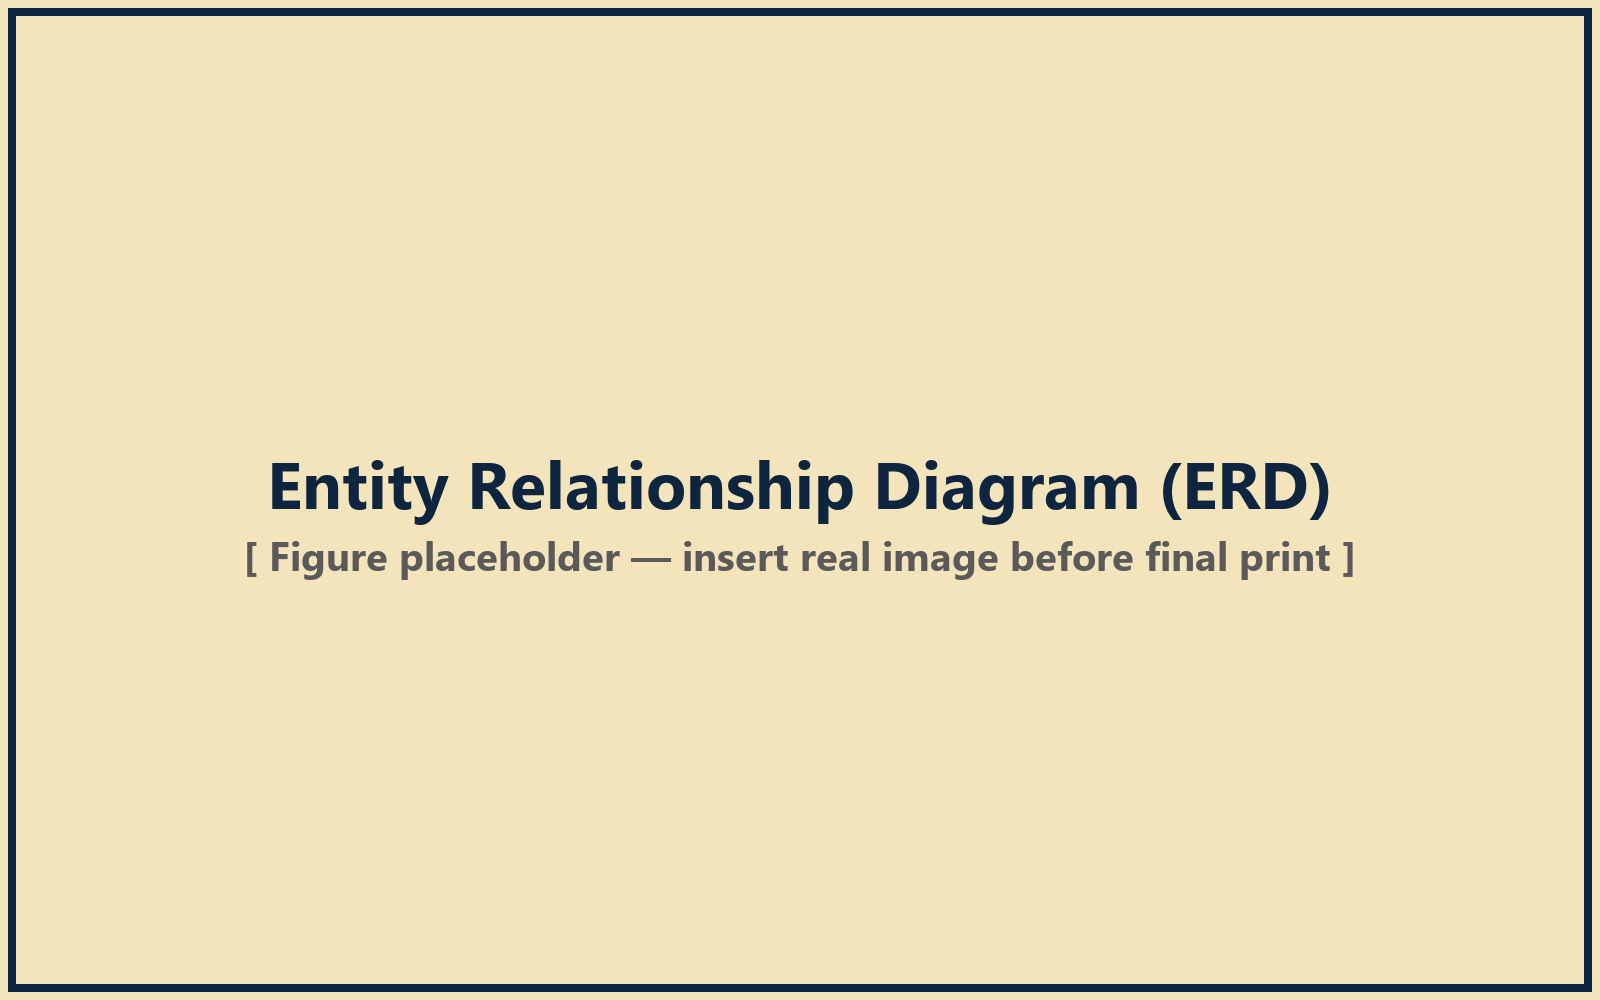
\includegraphics[width=0.9\textwidth]{figures/erd.png}
    \caption{Entity Relationship Diagram (ERD)}
    \label{fig:erd}
\end{figure}

\section{Frontend User Journeys and UI Design}
The Flutter application (`lib/presentation/`) is structurally divided by core domains. The User Interface (UI) follows a "Modern Heritage" design language—blending contemporary mobile UX patterns (glassmorphism, vibrant gradients) with culturally resonant typography and color palettes.

\subsection{Journey 1: Onboarding \& Authentication}
The user is first greeted by an animated Splash Screen, followed by an educational Walkthrough. The Authentication flow supports standard registration and OAuth. It intercepts deep links for email confirmation and password resets.

\begin{figure}[H]
    \centering
    \begin{minipage}{0.45\textwidth}
        \centering
        
\includegraphics[width=\linewidth]{figures/splash.png}
        \caption{Mobile Application Splash Screen}
        \label{fig:splash}
    \end{minipage}\hfill
    \begin{minipage}{0.45\textwidth}
        \centering
        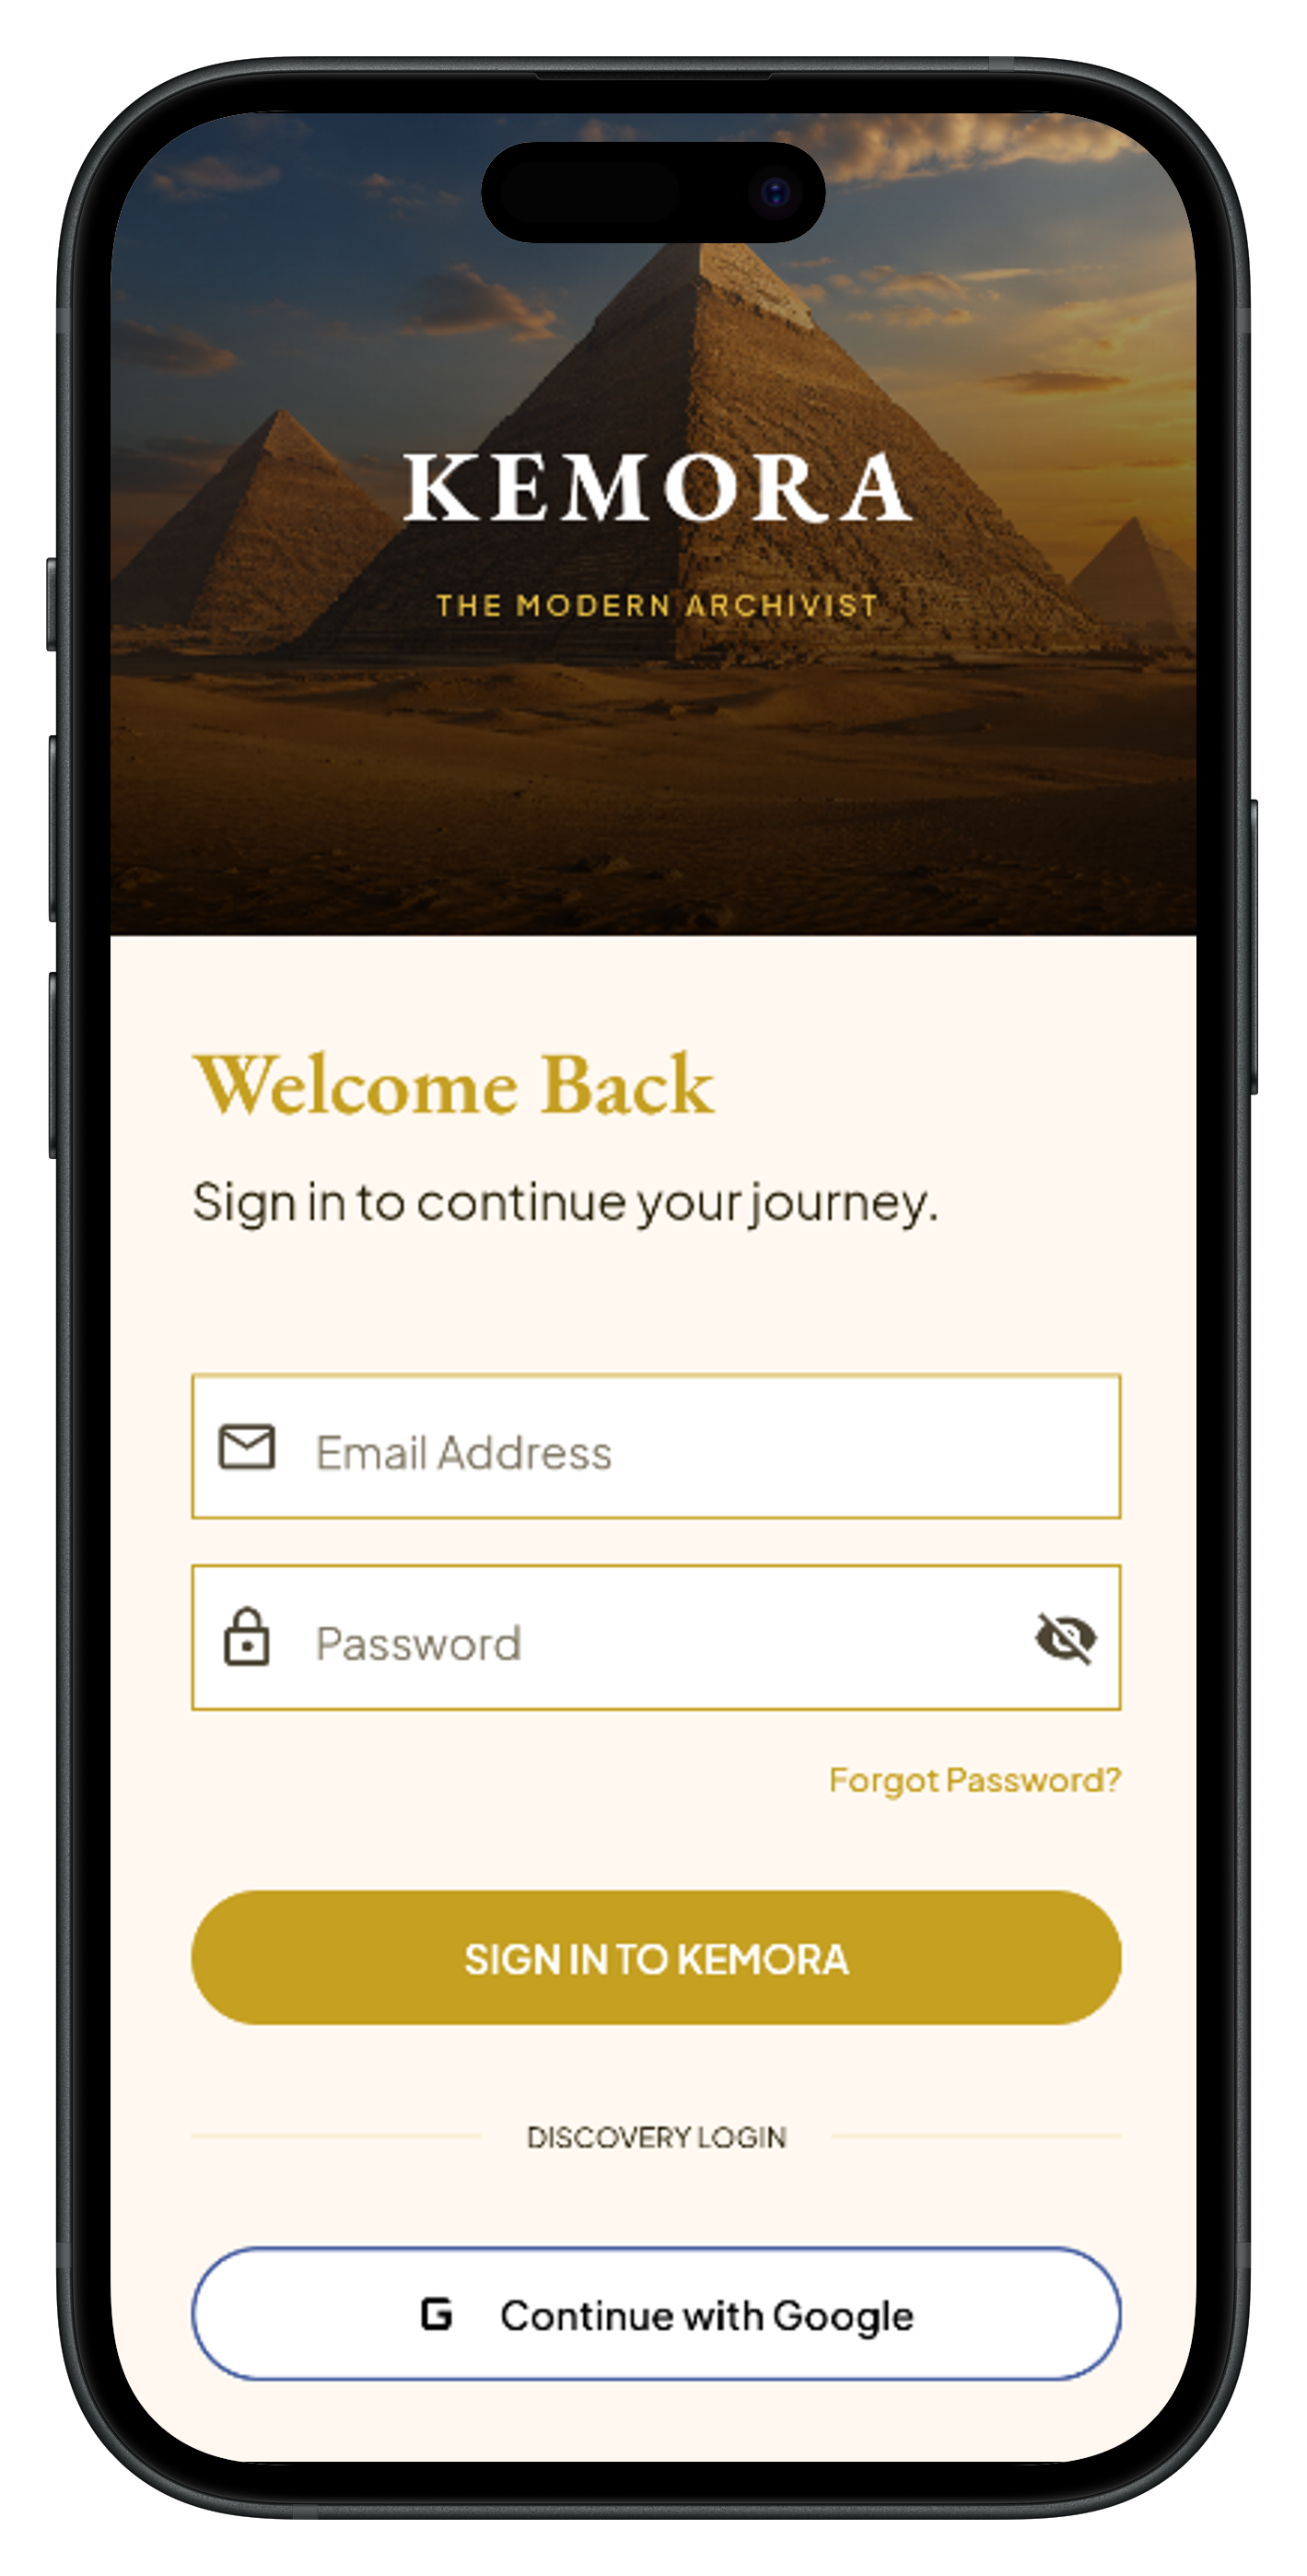
\includegraphics[width=\linewidth]{figures/login.png}
        \caption{Mobile Application Authentication Page}
        \label{fig:login}
    \end{minipage}
\end{figure}

\subsection{Journey 2: Main Dashboard \& Discovery}
The Home screen serves as the central hub, presenting personalized recommendations, top-rated destinations, and quick-action navigation via a custom floating tab bar.

\begin{figure}[H]
    \centering
    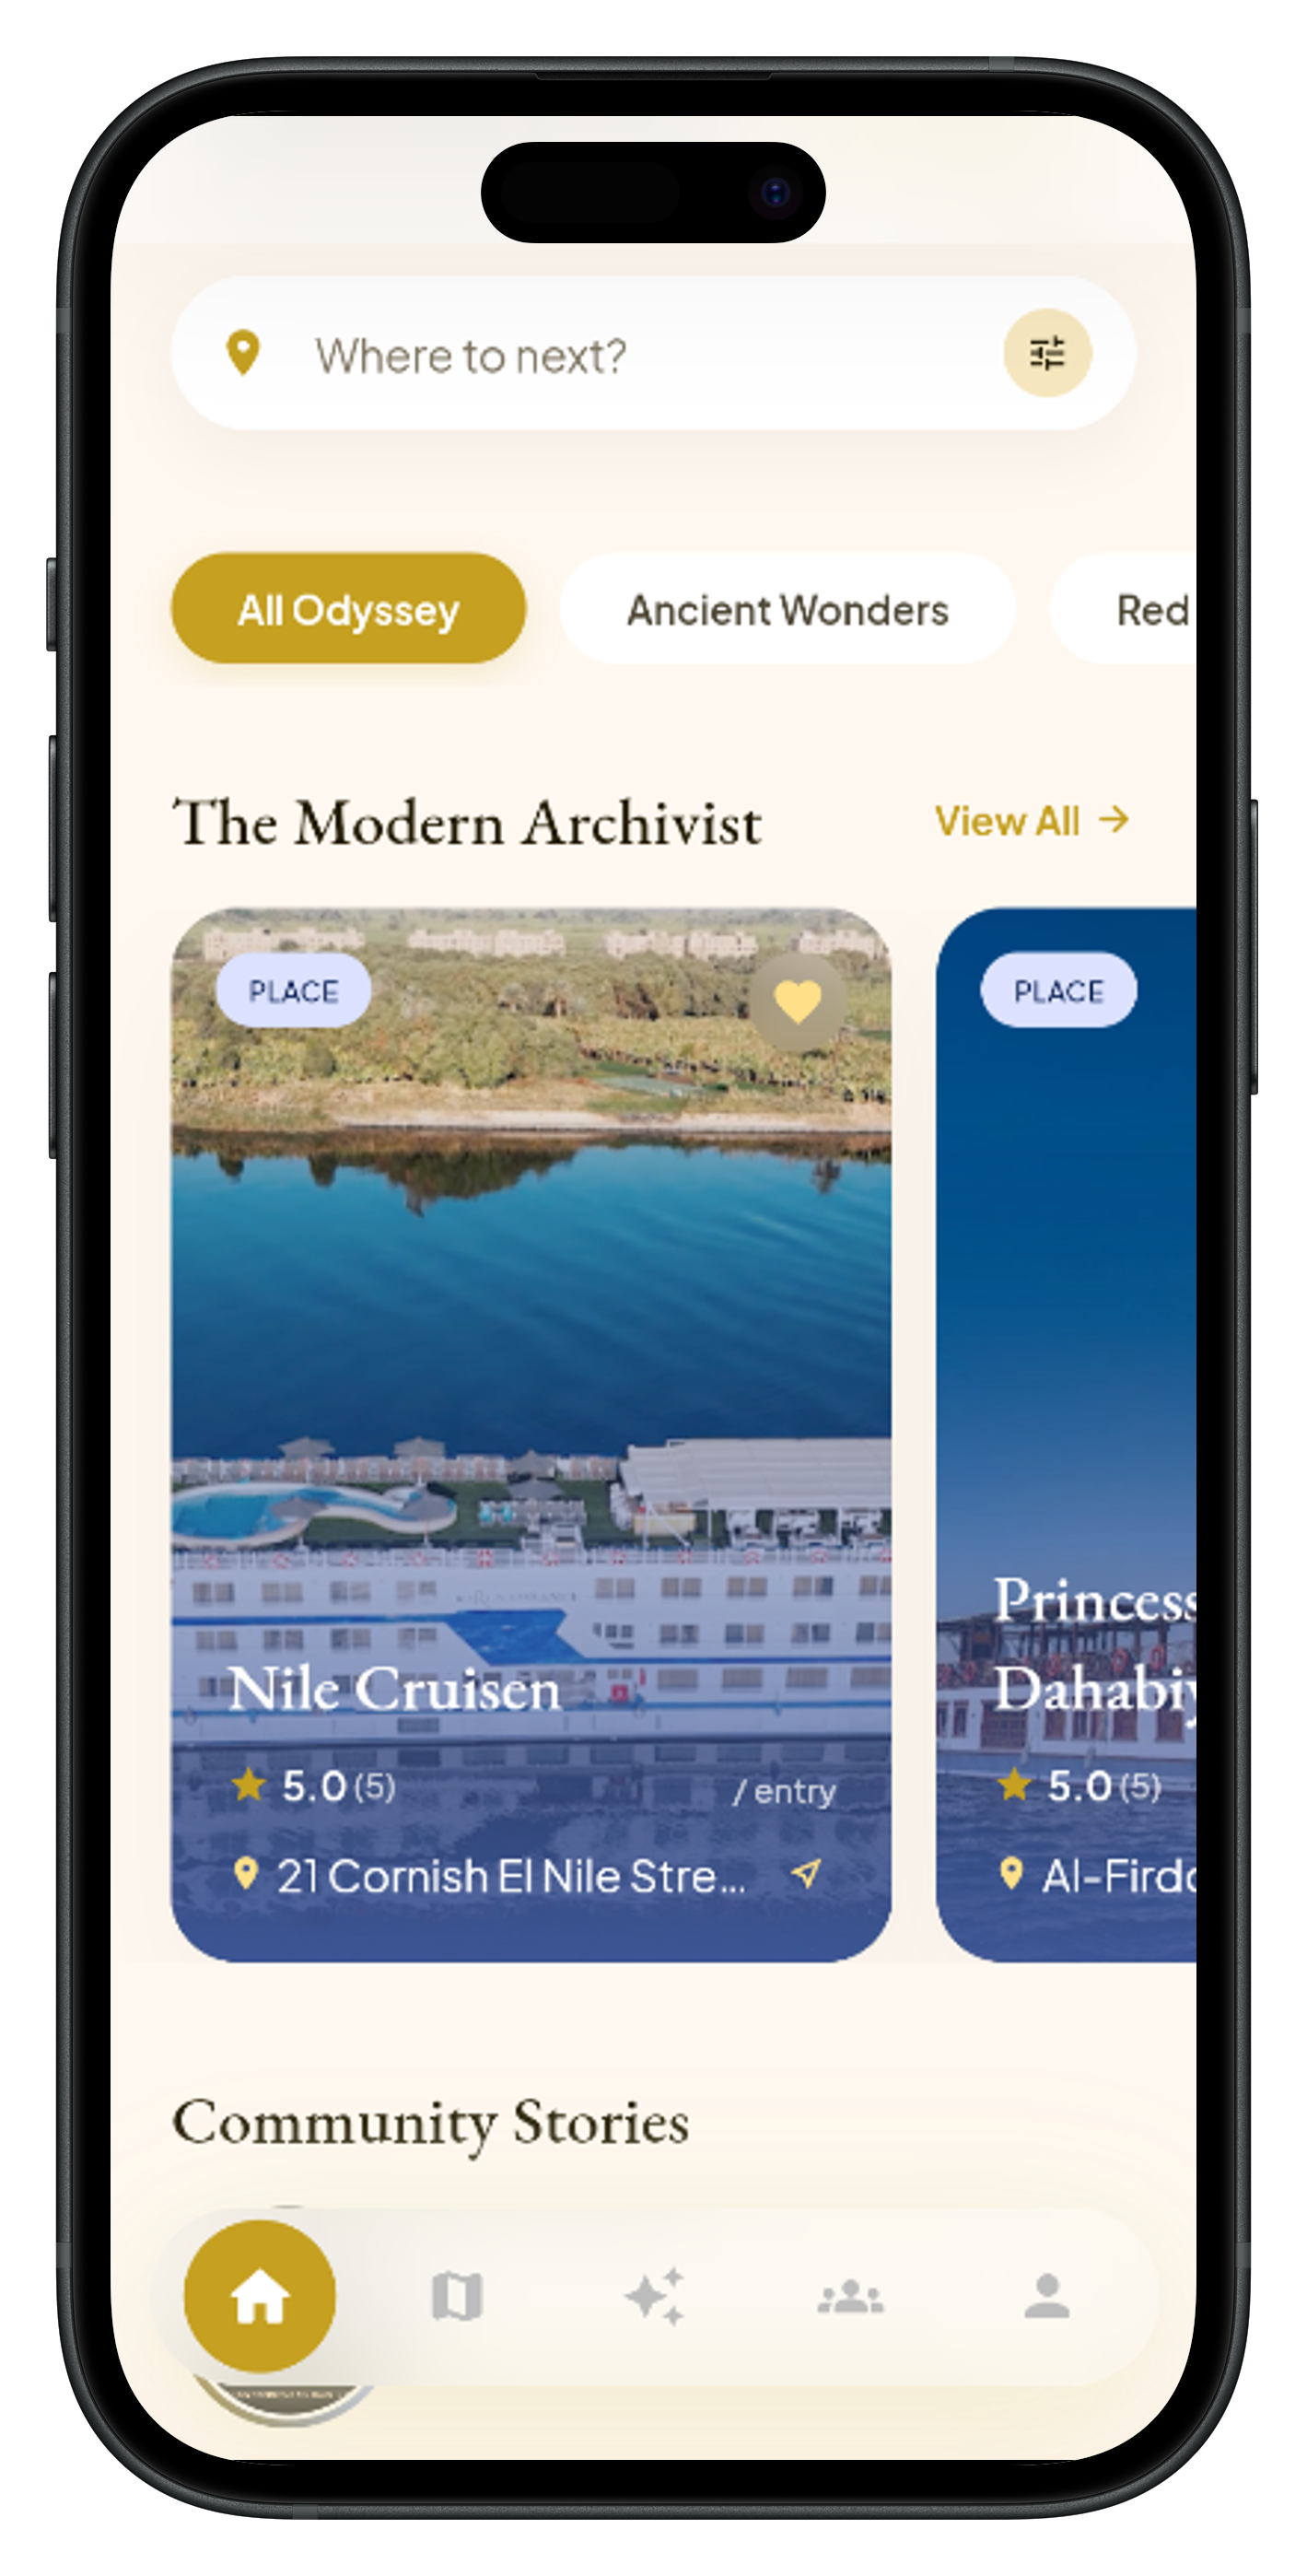
\includegraphics[width=0.45\textwidth]{figures/home.png}
    \caption{Mobile Application Home Page}
    \label{fig:home}
\end{figure}

\subsection{Journey 3: Explore \& Location Discovery}
Users can navigate an interactive map of Egyptian governorates. Selecting a governorate transitions to a detailed view listing sub-categories (Historical, Coastal, etc.) and individual Place detail screens.

\begin{figure}[H]
    \centering
    \begin{minipage}{0.3\textwidth}
        \centering
        
\includegraphics[width=\linewidth]{figures/map.png}
        \caption{Interactive Map}
        \label{fig:map}
    \end{minipage}\hfill
    \begin{minipage}{0.3\textwidth}
        \centering
        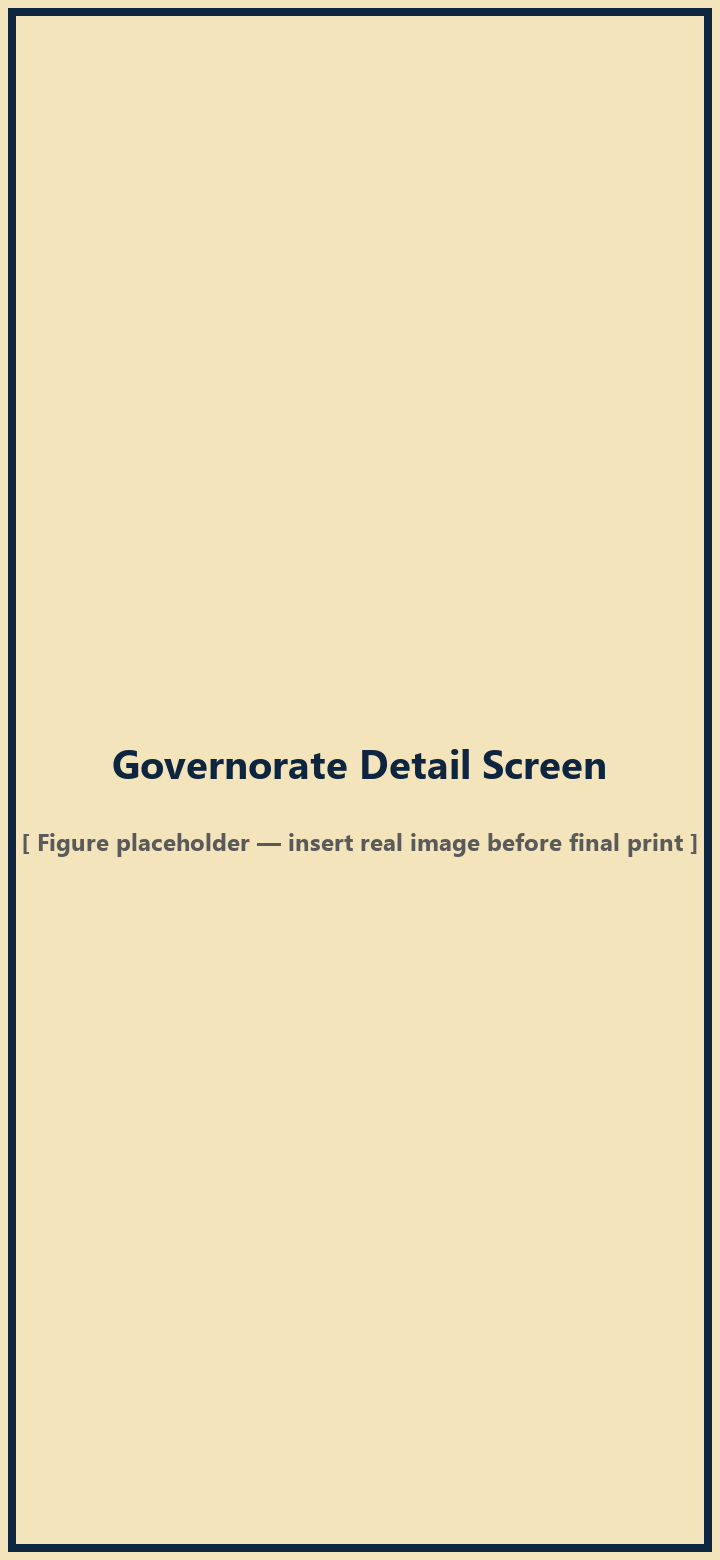
\includegraphics[width=\linewidth]{figures/gov_details.png}
        \caption{Governorate Details}
        \label{fig:gov_details}
    \end{minipage}\hfill
    \begin{minipage}{0.3\textwidth}
        \centering
        
\includegraphics[width=\linewidth]{figures/place_details.png}
        \caption{Place Details}
        \label{fig:place_details}
    \end{minipage}
\end{figure}

\subsection{Journey 4: Trip Planning \& AI Itinerary}
This is the flagship journey. Users input parameters into a multi-step questionnaire (`ai_step_questions_screen.dart`). The system displays a loading animation while negotiating with the backend AI. The result is a beautifully rendered, interactive timeline (`ai_itinerary_result_screen.dart`).

\begin{figure}[H]
    \centering
    \begin{minipage}{0.45\textwidth}
        \centering
        
\includegraphics[width=\linewidth]{figures/ai_questions.png}
        \caption{AI Trip Planner Questionnaire}
        \label{fig:ai_questions}
    \end{minipage}\hfill
    \begin{minipage}{0.45\textwidth}
        \centering
        
\includegraphics[width=\linewidth]{figures/ai_itinerary.png}
        \caption{AI Generated Itinerary Timeline}
        \label{fig:ai_itinerary}
    \end{minipage}
\end{figure}

\subsection{Journey 5: Social \& Community}
A familiar, vertically scrolling feed allows users to consume and produce content. Users can view detailed posts, engage in comment threads, and participate in direct real-time chats.

\begin{figure}[H]
    \centering
    \begin{minipage}{0.45\textwidth}
        \centering
        
\includegraphics[width=\linewidth]{figures/social_feed.png}
        \caption{Community Social Feed}
        \label{fig:social_feed}
    \end{minipage}\hfill
    \begin{minipage}{0.45\textwidth}
        \centering
        
\includegraphics[width=\linewidth]{figures/chat.png}
        \caption{Real-Time Messaging Interface}
        \label{fig:chat}
    \end{minipage}
\end{figure}

\subsection{Journey 6: Profile \& Gamification}
The Profile screen tracks the user's identity, displaying earned badges, total points, redeemed vouchers, and saved places.

\begin{figure}[H]
    \centering
    \begin{minipage}{0.45\textwidth}
        \centering
        
\includegraphics[width=\linewidth]{figures/profile.png}
        \caption{User Profile Screen}
        \label{fig:profile}
    \end{minipage}\hfill
    \begin{minipage}{0.45\textwidth}
        \centering
        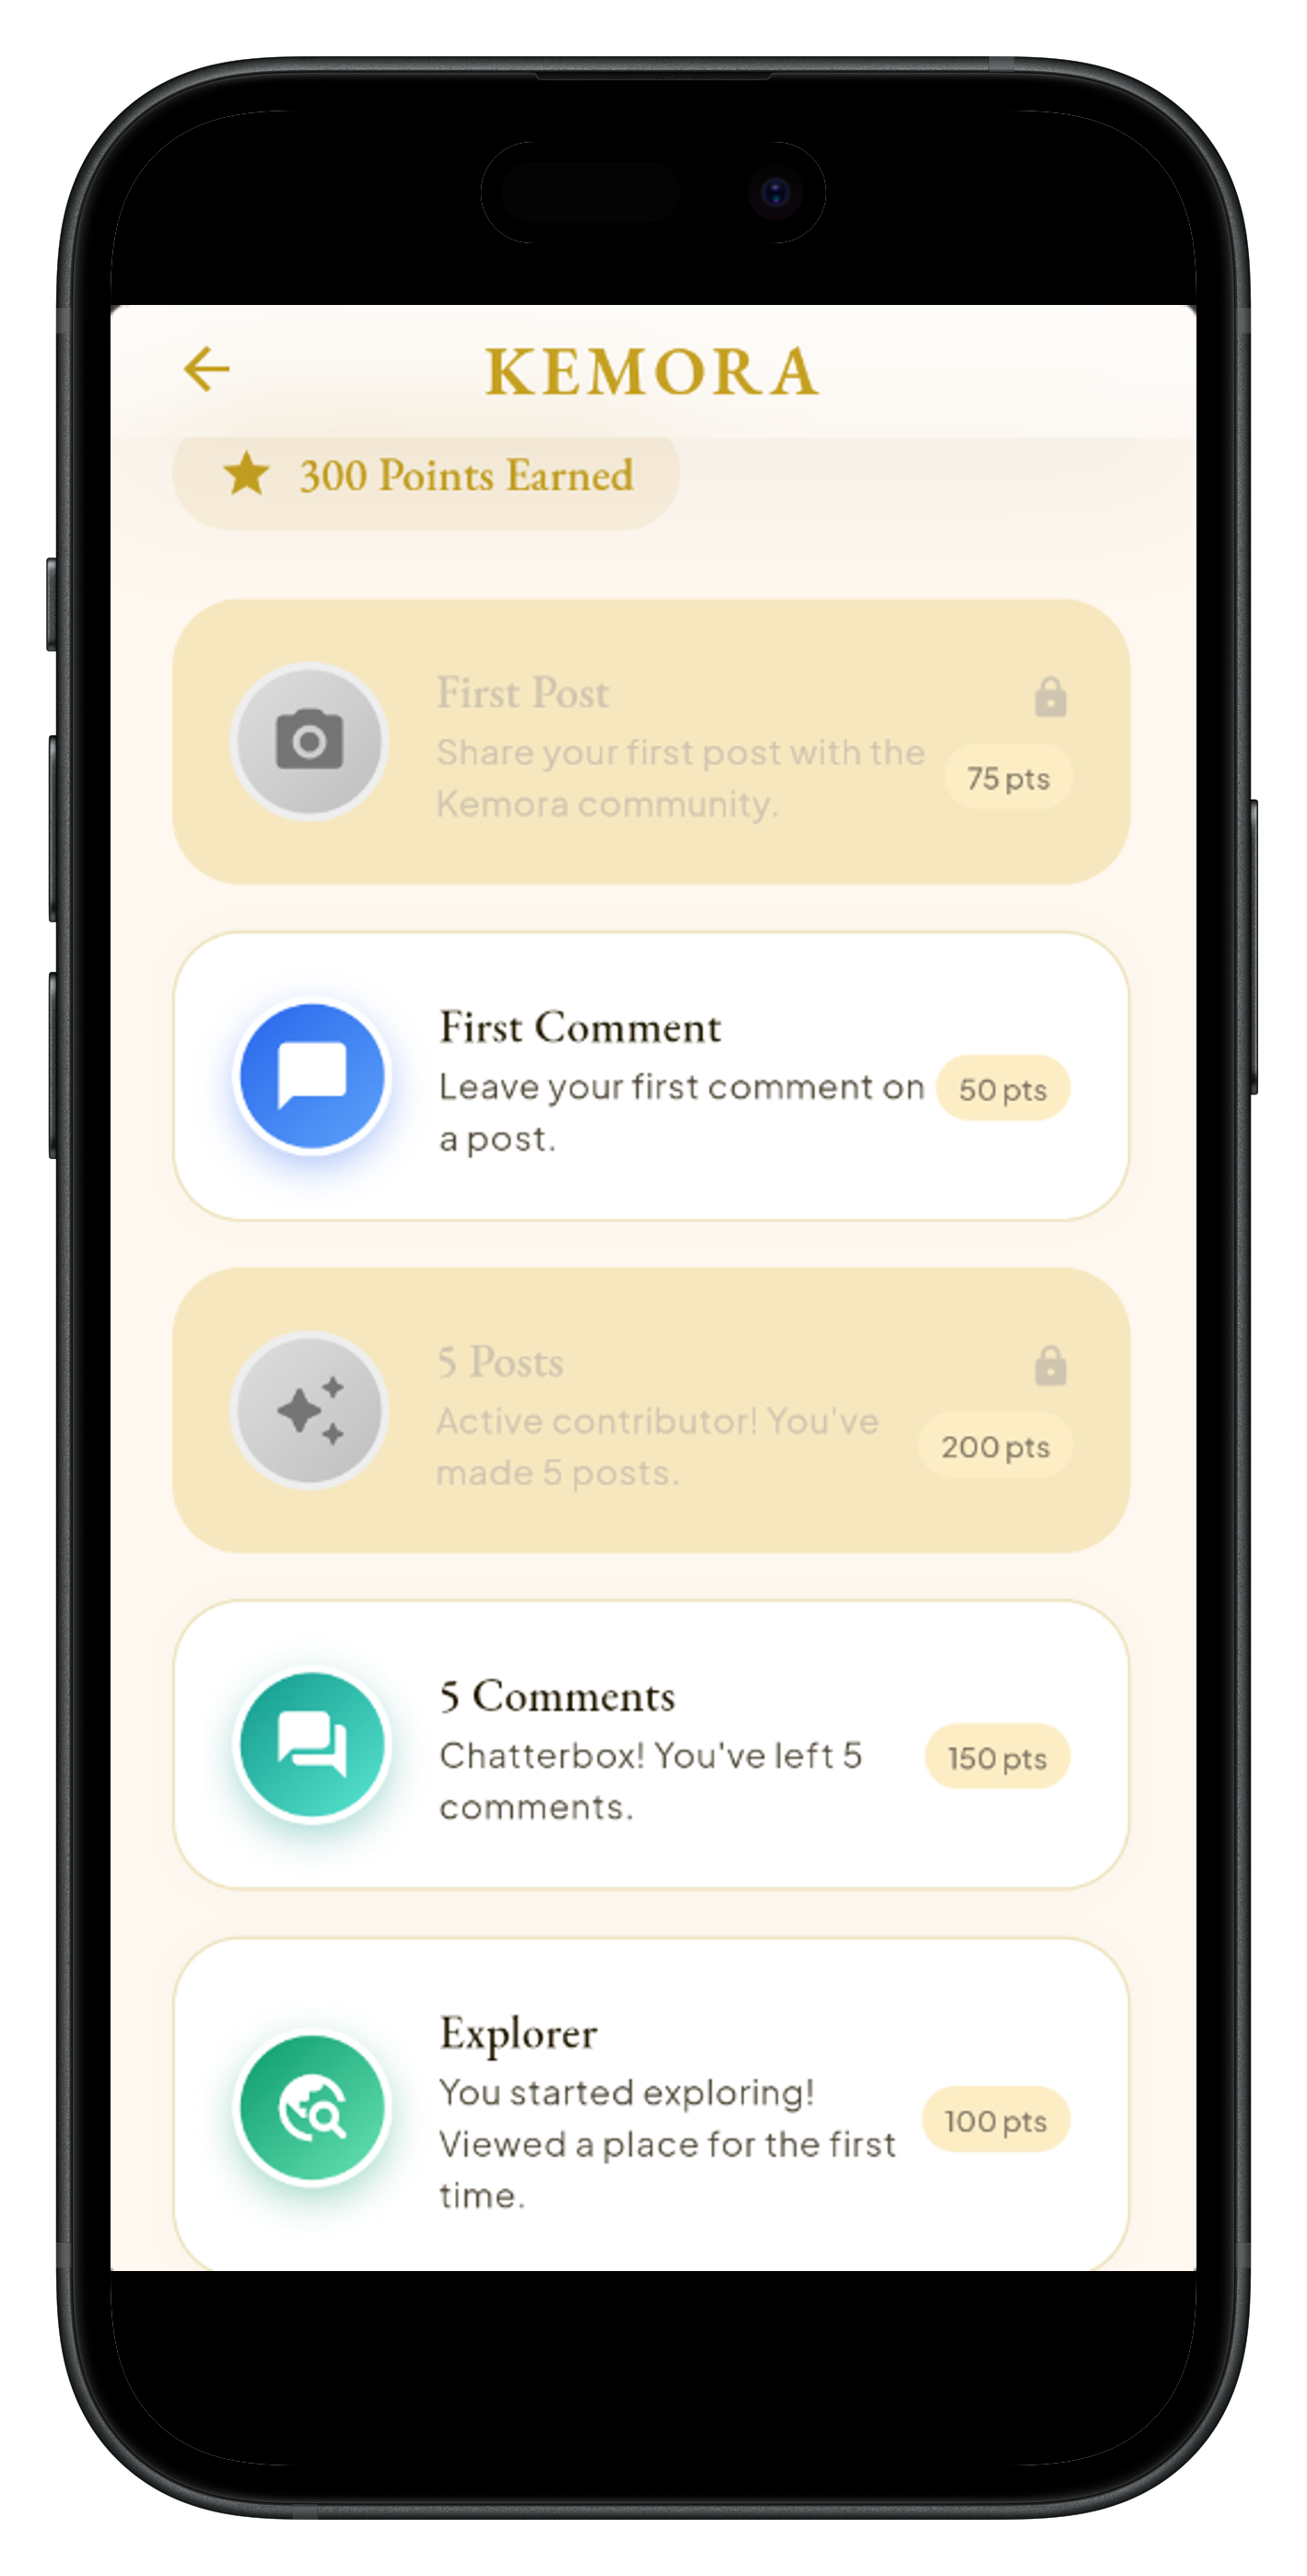
\includegraphics[width=\linewidth]{figures/badges.png}
        \caption{Gamification \& Badges Screen}
        \label{fig:badges}
    \end{minipage}
\end{figure}
